\title{Midterm 3 for Calculus-Based Physics: Electricity and Magnetism, with Answers}
\author{Dr. Jordan Hanson - Whittier College Dept. of Physics and Astronomy}
\date{\today}
\documentclass[10pt]{article}
\usepackage[a4paper, total={18cm, 27cm}]{geometry}
\usepackage{outlines}
\usepackage{graphicx}
\usepackage{amsmath}
\begin{document}
\maketitle

\section{Equations and constants}

\begin{enumerate}
\item Ohm's law: $V=iR$
\item Definition of magnetic flux: $\phi = \vec{B} \cdot \vec{A}$.  The units are T m$^2$, which is called a Weber, or Wb.
\item Faraday's Law: $emf = -N \frac{d\phi}{dt}$
\item Faraday's Law using \textbf{Inductance}, M: $emf = -M \frac{dI}{dt}$.
\item Faraday's Law using \textbf{Inductance}, M, with average change in current: $emf = -M \frac{\Delta I}{\Delta t}$.
\item Typically, we refer to \textit{mutual inductance} between two objects as $M$, and \textit{self inductance} as $L$.
\item Units of inductance: V s A$^{-1}$, which is called a Henry, or H.
\end{enumerate}

\section{Exercises}

\begin{enumerate}
\item \textbf{Chapter 13: Electromagnetic Induction}
\begin{enumerate}
\item
\begin{figure}[ht]
\centering
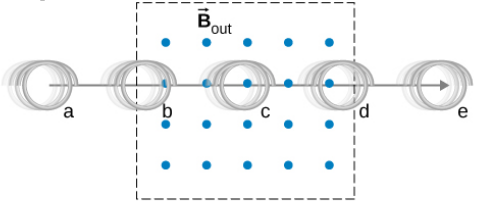
\includegraphics[width=0.4\textwidth]{magdamp.png}
\caption{\label{fig:flux1} A single loop of wire moves through a B-field.}
\end{figure}
A coil is moved through a magnetic field as shown in Fig. \ref{fig:flux1}. The field is uniform inside the rectangle and zero outside. What is the direction of the induced current (if one exists) and what is the direction of the magnetic force on the coil (if there is one) at each position shown?
\begin{itemize}
\item A: Current:$\rule{2cm}{0.15mm}$Force:$\rule{2cm}{0.15mm}$
\item B: Current:$\rule{2cm}{0.15mm}$Force:$\rule{2cm}{0.15mm}$
\item C: Current:$\rule{2cm}{0.15mm}$Force:$\rule{2cm}{0.15mm}$
\item D: Current:$\rule{2cm}{0.15mm}$Force:$\rule{2cm}{0.15mm}$
\item E: Current:$\rule{2cm}{0.15mm}$Force:$\rule{2cm}{0.15mm}$
\end{itemize}
\item In an AC generator, let $N$ be the number of coils, $A$ be the area of the coils, $\omega$ be the angular velocity of the coils, and $B$ be the magnetic field strength.  The induced emf is
\begin{equation}
emf = N\omega BA\sin(\omega t)
\end{equation}
For a generator design with $N=1000$, $B=0.1$ T, loops of area $10$ cm$^2$ (pay attention to units), turning at $\omega = 2\pi\times 100$ radians per second, (a) what is the maximum voltage?  (b) What is the maximum current through a 50 $\Omega$ resistor? \\ \vspace{2cm}
\clearpage
\item
\begin{figure}
\centering
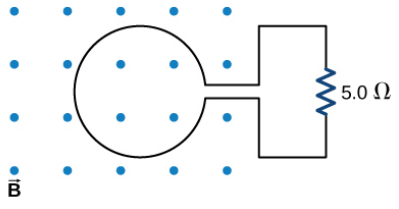
\includegraphics[width=0.3\textwidth]{loopsine.png}
\caption{\label{fig:flux2} A changing B-field through a loop of wire connected to a resistor.}
\end{figure} 
The magnetic field in Fig. \ref{fig:flux2} flows out of the page through a single ($N=1$) loop, and is tuned to follow the form
\begin{equation}
B(t) = B_0 e^{-at}\sin(2\pi f t)
\end{equation}
The loop has a radius $r$.  (a) In terms of the given variables, what is the induced voltage in the circuit? (b) If $B_0 = 0.1$ T, $r = 0.1$ m, and $f = 10^3$ Hz, what is the induced emf at $t=0$?  (c) What is the current through the resistor at $t=0$? (c) What is the induced emf as $t \to \infty$? \\ \vspace{4cm}
\end{enumerate}
\item \textbf{Chapter 14: Inductance}
\begin{enumerate}
\item What is (a) the rate at which the current though a 0.30-H coil is changing if an emf of 0.12 V is induced across the coil?\\ \vspace{1cm}
\item When a camera uses a flash, a fully charged capacitor discharges through an inductor. In what time must the 0.100-A current through a 2.00-mH inductor be switched on or off to induce a 500-V emf? (\textit{Hint: Solving for $\Delta t$}). \\ \vspace{1cm}
\item A coil with a self-inductance L carries a current $I(t) = I_0\ln(1+at)$ (A).  (a) What is the emf induced in the coil as a function of time? (b) If $L = 1.0$ mH, $a = 10^3$ Hz, and $I_0 = 2.0$ A, what is the voltage after 1.0 seconds?\footnote{\textit{Hint: $\frac{d}{dx} \ln(x) = x^{-1}$.}} \\ \vspace{4cm}
\end{enumerate}
\end{enumerate}

\end{document}
